Le pont H est une structure qui permet à la fois de \textbf{déterminer le sens de rotation} du moteur, mais également de \textbf{régler la vitesse de rotation} du moteur, notée $\omega_m$ dans les équations précédentes.\\

Le pont H est basé sur 4 interrupteurs dont les connexions vont permettre de changer le sens de la tension imposée au moteur, comme illustré à la Figure \ref{fig:h_bridge_principle}. Ce changement de sens de la tension permet de faire tourner le moteur DC dans les 2 sens de rotation possibles. Il est également possible de freiner le moteur en activant les 2 interrupteurs inférieurs (ou supérieurs) pour le court-circuiter. \\

\begin{figure}[!ht]
	\centering
	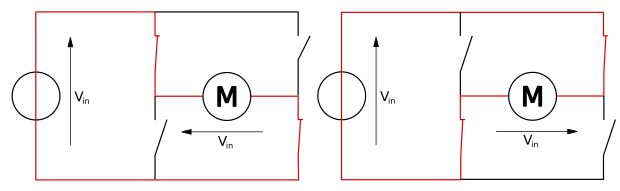
\includegraphics[width=.8\textwidth]{h_bridge_principle}
	\captionof{figure}{Principe de fonctionnement du pont H.}
	\label{fig:h_bridge_principle}
\end{figure}

Le réglage de la vitesse de rotation du moteur est réalisé par une modulation de la tension appliquée au moteur, appelée \textbf{modulation à largeur d'impulsion} (MLI). De façon générale, la source $V_{in}$ est une batterie et fournit une tension DC fixe dont il n'est pas possible de modifier la valeur, alors que cela est pourtant nécessaire pour pouvoir contrôler le moteur. La solution trouvée pour contourner ce problème consiste à moduler le rapport cyclique de la tension appliquée au moteur en connectant et déconnectant les switches du pont H. De cette façon, la valeur moyenne du signal (courbe rose sur la Figure \ref{fig:pwm_principle}) correspond à la valeur souhaitée (courbe verte sur la Figure \ref{fig:pwm_principle}). On arrive donc bien à générer une tension variable sur base d'une batterie fournissant une tension fixe.\\

En termes d'implémentation, le circuit du pont H est présenté à la Figure \ref{fig:h_bridge}. Les interrupteurs sont généralement implémentés sur base de transistors (bipolaires ou MOS) qui se trouveront ici dans le composant intégré (L293D). Les diodes mises en parallèle avec les interrupteurs sont des composants primordiaux pour assurer le bon fonctionnement du pont. En effet, le moteur étant constitué de bobinages qui présentent un comportement essentiellement inductif, le courant qui traverse ces bobinages ne pourra pas passer immédiatement à zéro lorsque l'on ouvre les interrupteurs. Les diodes sont donc là pour fournir un chemin au travers duquel peut passer ce courant, évitant ainsi d'endommager les interrupteurs.

\begin{minipage}[t]{.45\textwidth}
	\centering
	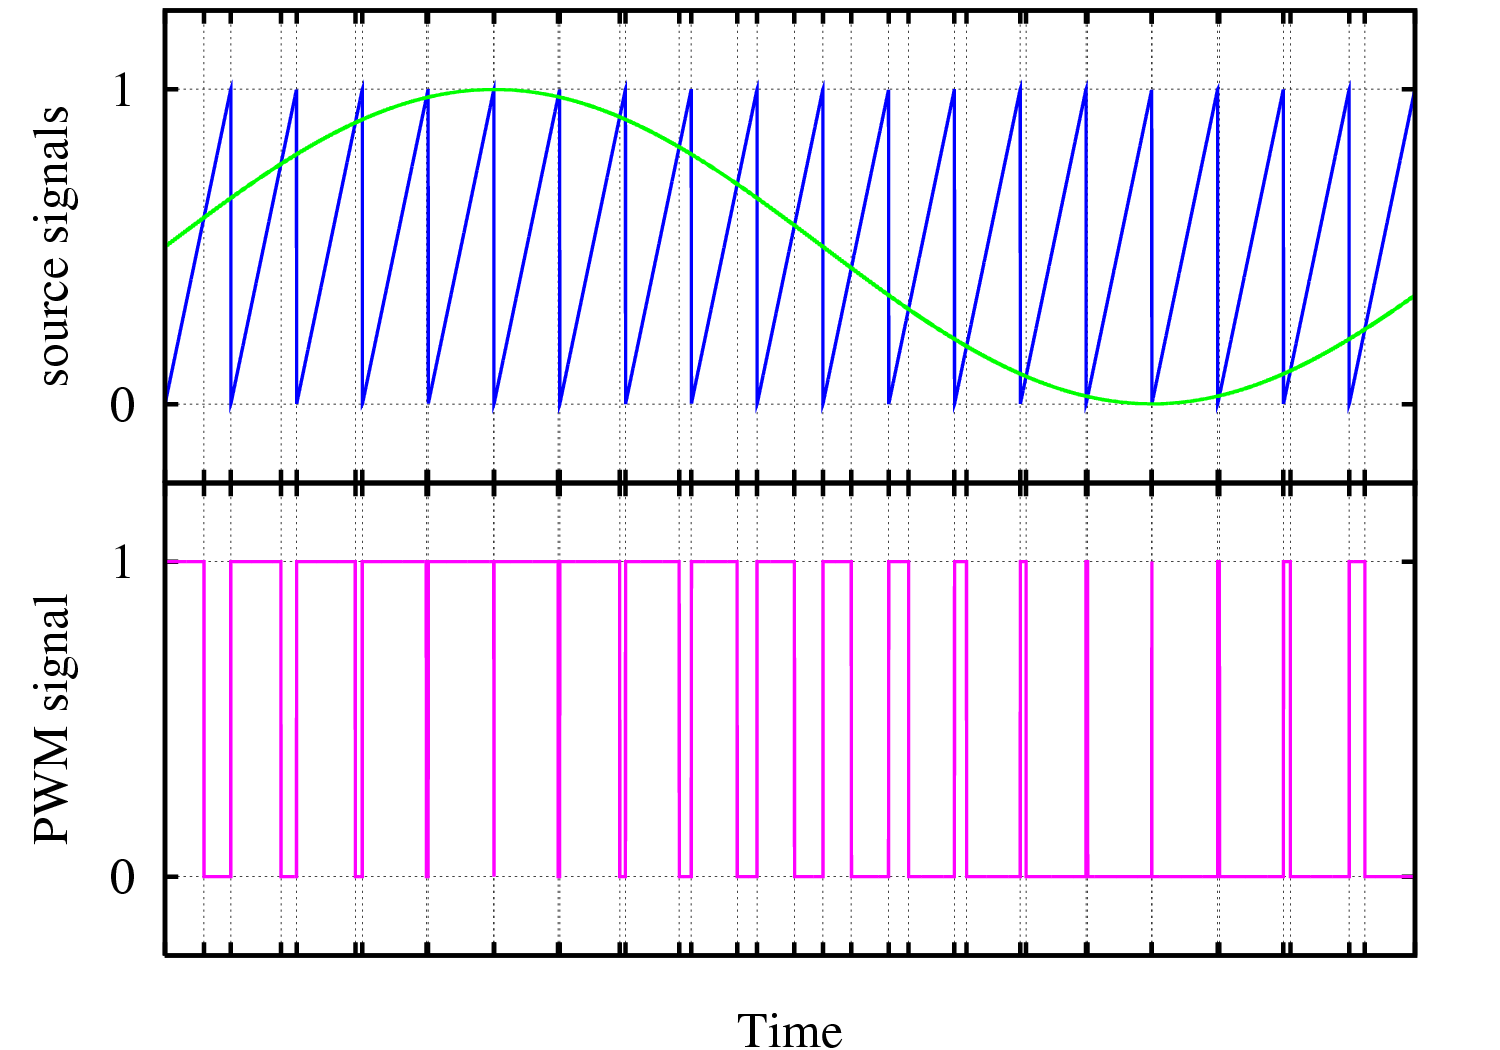
\includegraphics[width=\textwidth]{pwm_principle}
	\captionof{figure}{Modulation à largeur d'impulsion (MLI).}
	\label{fig:pwm_principle}
\end{minipage}
\hfill
\begin{minipage}[t]{.45\textwidth}
	\centering
	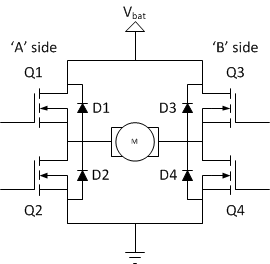
\includegraphics[width=\textwidth]{h_bridge}
	\captionof{figure}{Implémentation du pont H.}
	\label{fig:h_bridge}
\end{minipage}

